% arara: xelatex
% arara: xelatex
% arara: xelatex


\documentclass[thesis=M,english]{FITthesis}[2019/12/23]

%\usepackage[utf8]{inputenc} % LaTeX source encoded as UTF-8
% \usepackage[latin2]{inputenc} % LaTeX source encoded as ISO-8859-2
% \usepackage[cp1250]{inputenc} % LaTeX source encoded as Windows-1250

% \usepackage{subfig} %subfigures
% \usepackage{amsmath} %advanced maths
% \usepackage{amssymb} %additional math symbols

\usepackage{dirtree} %directory tree visualisation
\usepackage{url}
% \usepackage{svg}
% Smalltalk environment for listings package, available at https://gist.github.com/mattonem/f434605a35716bfabec9
\usepackage{color}
\usepackage{listings}
\usepackage{etoolbox}

\definecolor{stComment}{rgb}{0.5,0.5,0.5}
\definecolor{stString}{rgb}{0.58,0,0.82}
\definecolor{stKeywords}{rgb}{0.21,0.55,0.7}
\definecolor{stNumbers}{rgb}{.5,0,0}

\newtoggle{InString}{}% Keep track of if we are within a string
\togglefalse{InString}% Assume not initally in string
\newcommand*{\ColorIfNotInString}[1]{\iftoggle{InString}{#1}{\color{stNumbers}#1}}%
\newcommand*{\ProcessQuote}[1]{#1\iftoggle{InString}{\global\togglefalse{InString}}{\global\toggletrue{InString}}}%

\lstdefinelanguage{Smalltalk}{
  basicstyle={\small\ttfamily},
  keywordstyle=\color{stKeywords},
  commentstyle=\color{stComment},
  stringstyle=\color{stString},
  alsoletter=\#,
  identifierstyle=\idstyle, 
  showstringspaces=false,
  morekeywords={true,false,self,super,nil},
  sensitive=true, 
  morecomment=[s]{"}{"}, 
  morestring=[d]', 
  style=SmalltalkStyle,
  tabsize=2,
}


\makeatletter%
\newcommand*\idstyle[1]{%
  \expandafter\id@style\the\lst@token{#1}\relax%
}
\def\id@style#1#2\relax{%
  \ifnum\pdfstrcmp{#1}{\#}=0%
  \ttfamily\color{stString} \the\lst@token%
  \else%
  \edef\tempa{\uccode`#1}%
  \edef\tempb{`#1}%
  \ifnum\tempa=\tempb%
  \ttfamily\color{blue} \the\lst@token%
  \else%
  \the\lst@token%
  \fi%
  \fi%
}

\lstdefinestyle{SmalltalkStyle}{ 
  literate=%
  {^}{{$\uparrow$}}1% 
  % {"}{{{\ProcessQuote{"}}}}1% Disable coloring within double quotes
  % {'}{{{\ProcessQuote{'}}}}1% Disable coloring within single quote
  {0}{{{\ColorIfNotInString{0}}}}1%
  {1}{{{\ColorIfNotInString{1}}}}1%
  {2}{{{\ColorIfNotInString{2}}}}1%
  {3}{{{\ColorIfNotInString{3}}}}1%
  {4}{{{\ColorIfNotInString{4}}}}1%
  {5}{{{\ColorIfNotInString{5}}}}1%
  {6}{{{\ColorIfNotInString{6}}}}1%
  {7}{{{\ColorIfNotInString{7}}}}1%
  {8}{{{\ColorIfNotInString{8}}}}1%
  {9}{{{\ColorIfNotInString{9}}}}1%
} 

% % list of acronyms
% \usepackage[acronym,nonumberlist,toc,numberedsection=autolabel]{glossaries}
% \iflanguage{czech}{\renewcommand*{\acronymname}{Seznam pou{\v z}it{\' y}ch zkratek}}{}
% \makeglossaries

\department{Department of Theoretical Computer Science}
\title{SimpleObjectMachine implementation}
\authorGN{Rudolf} %author's given name/names
\authorFN{Rovňák} %author's surname
\author{Rudolf Rovňák} %author's name without academic degrees
\authorWithDegrees{Bc. Rudolf Rovňák} %author's name with academic degrees
\supervisor{Ing. Petr Máj}
\acknowledgements{THANKS (remove entirely in case you do not with to thank anyone)}
\abstractEN{Summarize the contents and contribution of your work in a few sentences in English language.}
\abstractCS{V n{\v e}kolika v{\v e}t{\' a}ch shr{\v n}te obsah a p{\v r}{\' i}nos t{\' e}to pr{\' a}ce v {\v c}esk{\' e}m jazyce.}
\placeForDeclarationOfAuthenticity{Prague}
\keywordsCS{Replace with comma-separated list of keywords in Czech.}
\keywordsEN{Replace with comma-separated list of keywords in English.}
\declarationOfAuthenticityOption{1} %select as appropriate, according to the desired license (integer 1-6)
% \website{http://site.example/thesis} %optional thesis URL


\begin{document}

% \newacronym{CVUT}{{\v C}VUT}{{\v C}esk{\' e} vysok{\' e} u{\v c}en{\' i} technick{\' e} v Praze}
% \newacronym{FIT}{FIT}{Fakulta informa{\v c}n{\' i}ch technologi{\' i}}

% \setsecnumdepth{part}
\setcounter{secnumdepth}{3}
\chapter{Introduction}
In the last decades, a trend of dynamic programming languages \footnote{Not to be confused with \textit{dynamically typed programming languages.}} has been on the rise.
As opposed to static programming languages (usually compiled) dynamic ones offer a higher level of abstraction and allow faster and less error-prone development.
Dynamic languages move a lot of actions traditionally done during compile-time to run-time. This creates the need for another layer, \textit{a runtime environment}.

My goal in this diploma thesis is to implement a process virtual machine for a programming language called SOM, or Simple Object Machine. 
It is a dynamic, object-oriented programming language based on Smalltalk. It was originally implemented at University of Århus in Denmark to teach
object oriented VMs \cite{som-github}. There are several implementations in various programming languages, ranging in speed, optimizations etc.

My main focus in my work will be the clarity of implementation over performance. 

\chapter{Analysis and design}
\textit{Simple Object Machine} (SOM) is a minimal Smalltalk dialect used primarily for teaching construction of virtual machines. Key characteristics
according to official website (\cite{som-github}) are:
\begin{itemize}
	\item clarity of implementation over performance,
	\item common language features such as: objects, classes, closures, non-local returns
	\item interpreter optimizations, threading, garbage collectors are different
		across various implementations.
\end{itemize}

\section{Grammar}
To implement a parser for the language, I decided to use ANTLR. I will demonstrate language features and design on the following ANTLR grammar
for SOM. For the sake of brevity, I ommited terminal symbols from the complete grammar as they are self-explanatory. All the terminal symbols
in this grammar are named in uppercase letters.

\begin{verbatim}
	grammar SOM;

	classDefinition:
		IDENTIFIER EQUALS superclass
		instanceFields method*
		(SEPARATOR classFields method*) ?
		CLOSE_PAR
	;
	superclass: IDENTIFIER? OPEN_PAR;
	instanceFields: (VBAR variable* VBAR)?;
	classFields: (VBAR variable* VBAR)?;
	method: pattern EQUALS methodBlock;
	methodBlock: OPEN_PAR blockContents? CLOSE_PAR;
	blockContents:
		(VBAR localDefinitions VBAR)?
		blockBody;
	localDefinitions: variable*;
	blockBody: 
		  RETURN result
		| expression (PERIOD blockBody?)?;
	result: expression PERIOD?;
	expression: assignation | evaluation;
	assignation: assignments evaluation;
	assignments: assignment+;
	assignment: variable ASSIGN;
	evaluation: primary messages?;
	primary: variable | nestedTerm | nestedBlock | literal;
	messages:
		  unaryMessage+ binaryMessage* keywordMessage?
		| binaryMessage+ keywordMessage?
		| keywordMessage;
	unaryMessage: IDENTIFIER;
	binaryMessage: binarySelector binaryOperand;
	binaryOperand: primary unaryMessage*;
	keywordMessage: (KEYWORD formula)+;
	formula: binaryOperand binaryMessage*;
	nestedTerm: OPEN_PAR expression CLOSE_PAR;
	nestedBlock:
		NEW_BLOCK blockPattern? blockContents? CLOSE_BLOCK;
	blockPattern: blockArgs VBAR;
	blockArgs: (COLON argument)+;
	variable: IDENTIFIER;
	pattern: unaryPattern | keywordPattern | binaryPattern;
	unaryPattern: unarySelector;
	unarySelector: IDENTIFIER;
	binaryPattern: binarySelector argument;
	keywordPattern: (KEYWORD argument)+;
	binarySelector: 
		VBAR | PLUS | MINUS | EQUALS | MULT | DIV | MOD |
		GREATER | GREATER_EQ | LESS | LESS_EQ;
	argument: variable;
	literal: literalNumber | literalString | literalArray | literalSymbol;
	literalNumber: MINUS? (INTEGER | DOUBLE);
	literalString: STRING;
	literalArray: POUND NEW_BLOCK literal* CLOSE_BLOCK;
	literalSymbol: POUND (STRING | selector);
	selector: binarySelector | keywordSelector | unarySelector;
	keywordSelector: KEYWORD+;
\end{verbatim}

\section{Class definition}
\begin{figure}[h!]
	\centering
	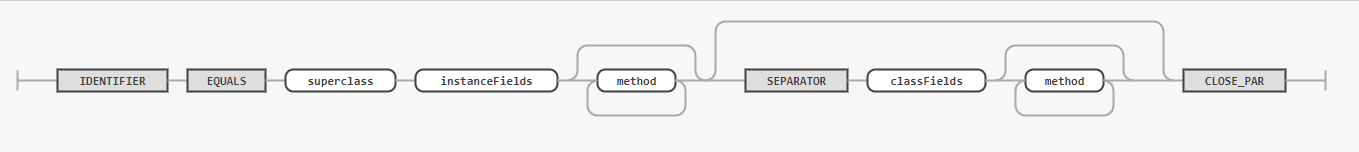
\includegraphics[width=\textwidth]{media/grammar/classDefinition_rrd.png}
	\caption{Railroad diagram for \texttt{classDefinition} rule.}
	\label{fig:classDefinition_rrd}
\end{figure}

\begin{lstlisting}[language=Smalltalk]
	SimpleHello = (
		| name |

		setName: aString (
			name := aString
		)

		printGreeting (
			('Hello, ', name) print
		)
	)
\end{lstlisting}

Syntax for class definition follows the official SOM grammar. The language supports single inheritance as apparent from the use
of \texttt{subclass} token in the grammar. Not every class has explicitly specified superclass, therefore the actual identifier in
the rule is optional.

Declaration of instance side fields follows, denoted by vertical bars. This token itself can be empty. Instance side methods definitions
are next. Further details on \textit{methods} and \textit{messages} in SOM are discussed in TODO. % TODO: add a link to section on methods
Same syntax is used for class side fields and methods separated by a special token.

\subsection{Variables}
In Smalltalk, a variable is defined as \textit{``a dynamically modifiable association (binding) of either a name
or an index to a value. Each distinct variable has exactly one name (or index)''}\cite{smalltalk-essentials}.

A value of a named variable can be any object. Indexed variables are at the core also just an object. They
represent an ordered sequence of objects as a single value. Example of those are arrays or Strings. Actual
indices are always strictly positive (greater than zero), meaning the first element of an array corresponds
to index of value one. This is standard in Smalltalk dialects, although uncommon in C-like languages. Retrieving
the values belonging to an index is done via sending a message to the encapsualting object.

When creating a new variable, it is assigned a special value \texttt{nil}, meaning the variable is empty. This
special value can also be explicitly assigned to a variable at any point.

\subsubsection{Variable name scoping}
Every variable has its scope, which determines the visibility of the variable. SOM follows the rules of Smalltalk
when it comes to scoping, as defined in \cite{smalltalk-essentials}:

\begin{itemize}
	\item \textbf{Local variables} are accessible within the method or code block in which they are defined.
	\item \textbf{Formal method arguments} are accessible by the method wherein they are defined.
	\item \textbf{Formal block arguments} are accessible by the block wherein they are defined.
	\item \textbf{Instance variables} are accessible within all methods of a given object. Each object
		has its own instances of these variables.
	\item \textbf{Class variables} are accessible by all objects that are instances of the class or its
		subclasses. All the objects share the same instance of this variable.
	\item \textbf{Global variables} are accessible everywhere.
\end{itemize}



\section{Primitives}
Even though SOM is purely object oriented, in order toto get any actual computations done, there is a point where
some virtual machine primitives must be invoked. Following things are therefore implemented as primitives:
\begin{itemize}
	\item memory allocation (\texttt{new} message),
	\item bitwise operations,
	\item integer arithmethics (\texttt{+}, \texttt{-}, \texttt{=} etc.),
	\item array accessing (\texttt{at:}, \texttt{at:put:})
\end{itemize}

\section{Methods and messages}
As the SOM language is based on Smalltalk, the concept of messages (and the link to methods) is crucial to understand.
\textit{``The only way to invoke a method is to send a message -- which necessarily involves dynamic binding
(by name) of message to method at runtime (and never at compile time). The internals of an object are not
externally accessible, ever -- the only way to access or modify an object's internal state is to send it
a message''} \cite{smalltalk-essentials}.

Execution of an invoked method ends with the execution of the last expression in it. Every method implicitly
returns \texttt{self} (a reference to the object on which the method is invoked). Explicit return of a value
is done with a special token \texttt{\^}. Execution of an expression preceeded by this token will exit the method.

The \cite{pharo-by-example} defines a helpful terminology for message passing:
\begin{itemize}
	\item A message is composed of the message \textit{selector} and the optional message arguments.
	\item Every message must be sent to its \textit{receiver}.
	\item Message and its receiver together will be referred to as \textit{message send}.
\end{itemize}

There are three types of messages (as defined in other Smalltalk dialects, Pharo as an example of one).

\textbf{Unary messages} are sent to an object without any additional information (argument). In the following
example, a unary message \texttt{size} is sent to a string object.
\begin{lstlisting}[language=Smalltalk]
	'hello' size "Evaluates to 5"
\end{lstlisting}

\textbf{Binary messages} are a special type of messages that require exactly one argument. The selector
of a binary message can only consist of a sequence of one or more characters from the set: +, -, *, /,
\&, =, \textless, \textgreater, |, ~ and @. A very simple example of usage of binary messsage are arithmetic operations.
\begin{lstlisting}[language=Smalltalk]
	3 + 4 "Evaluates to 7"
\end{lstlisting}

\textbf{Keyword messages} require one or more arguments. From the syntactic standpoint, they consist of
multiple keywords, each ending in colon (:). When sending a message, each keyword is followed by an argument.
Note, that a keyword message taking one argument is different to a binary message.
\begin{lstlisting}[language=Smalltalk]
	| numbers |
	numbers := #(1 2 3 4 5). "Simple array"
	"Sending a keyword message at:put: to an object of class Array"
	numbers at: 1 put: 6 "numbers is now #(6 2 3 4 5)"
\end{lstlisting}

When composing messages of various types, there are precedence rules (as defined for Pharo in \cite{pharo-by-example}):
\begin{itemize}
	\item Unary messages are sent first, followed by binary messages. Keyword messages are sent last.
	\item Messages in parentheses are sent before other messages.
	\item Messages of the same kind are evaluated from left to right.
\end{itemize}

These simple rules permit a very natural way of sending messages, as demonstrated on the next example.
First, a simple array is created. Then, a unary message \texttt{last} is evaluated, returning the last
element of the array. After that, binary message \texttt{+} is evaluated (to 2 in this example). Finally,
keyword message \texttt{at:put:} is sent to an array, putting number 5 on the second position in an array.
\begin{lstlisting}[language=Smalltalk]
	| numbers |
	numbers := #(1 2 3 4 5).
	numbers at: 1 + 1 put: numbers last.
	"numbers at: (1 + 1) put: (numbers last)"
\end{lstlisting}

Next example demonstrates sending messages from left to right when all of them are of the same type.
\begin{lstlisting}[language=Smalltalk]
	| numbers |
	numbers := #(1 2 3 4 5)
	numbers last asString print
	"This is equivalent to the following message sends"
	((numbers last) asString) print
\end{lstlisting}

There is a downfall to the simplicity of these rules. Arithmethic operations are all just a simple binary
message sends, therefore to ensure proper precedence, it is necessary to use parentheses.

\section{Blocks}
Blocks provide a mechanism to defer the execution of expressions \cite{pharo-by-example}.
Blocks can be treated as an object -- they can be assigned to variables and
passed as arguments. 

Blocks can also accept parameters -- they are denoted with a leading colon. Parameters are separated from the body
of the block by a vertical bar. Local variables can also be declared inside a block.

Block is executed by sending it a message \texttt{value}. However, this is a unary message and there is no way
to pass parameters to a block. To solve this problem, a keyword message \texttt{value:} is implemented. So far, this
gives a user to pass only one parameter to a block. To mitigate this issue, there are two posibilities. The first one
is to implement a keyword message for every number of parameters (for example \texttt{value:value:}, 
\texttt{value:value:value:}). While this approach is simple, readable and relatively easy to implement for low
numbers of parameters, it is impossible for this solution to be exhaustive and the code using very long keyword
messages would be bloated.

Another approach would be to implement a keyword message \texttt{value:} with an argument of array type. This would
permit to use arbitrary number of arguments, though it would require to create arrays of objects before passing them
to a block, which could impact readability and clarity of the code. In order to combine pros and cons of these 2
approaches, I have decided to follow the implementation in Pharo according to \cite[p.~65]{pharo-by-example}. 
There are keyword methods implemented for up to four parameters (\texttt{value:}, \texttt{value:value:}). For more
than four parameters, a special keyword message \texttt{valueWithArguments:} is implemented, where an array of
parameters is expected.

\begin{figure}
	\caption{Example of blocks usage in SOM.}
	\begin{lstlisting}[language=Smalltalk]
		| b0 b1 b2 b3 |
		b0 := [ 1 + 2 ].
		b1 := [ :x | x * x ].
		b2 := [ :x :y | x * y ].
		b3 := [ :x :y :z | x + y + z ].
		"Evaluating the blocks"
		b0 value. "Returns 3"
		b1 value: 3. "Returns 9"
		b2 value: 2 value: 8. "Returns 16"
		"Message valueWithArguments: can be used with any number of parameters"
		b3 valueWithArguments: #(1 2 3). "Returns 6
		"The next expression is functionally identical to the previous one"
		b3 value: 1 value: 2 value: 3.
	\end{lstlisting}
\end{figure}

\section{Expressions}
According to \cite{smalltalk-essentials}, \textit{an expression is a segment of code in a body of executable code
that can be evaluated to yield a value as a result of its execution.} As seen from the grammar snippet on figure
TODO, expressions are recursive structures.

\begin{figure}
	\begin{verbatim}
	expression: assignation | evaluation;
	assignation: assignments evaluation;
	assignments: assignment+;
	assignment: variable ASSIGN;
	evaluation: primary messages?;
	primary: variable | nestedTerm | nestedBlock | literal;
	messages:
		  unaryMessage+ binaryMessage* keywordMessage?
		| binaryMessage+ keywordMessage?
		| keywordMessage;
	\end{verbatim}
\end{figure}

Syntactically, an expression can consist of \cite{smalltalk-essentials}:
\begin{itemize}
	\item literal,
	\item variable/constant reference,
	\item message send,
	\item nested expression.
\end{itemize}

\section{Control structures}
In Smalltalk, there are no built-in control structures, unlike for example C++ or Java. SOM follows this principle
from Smalltalk, therefore there are no grammatical rules for branching or loops.

The way controlling the flow of program works in SOM is, again, by sending messages. One big advantage of this 
approach is that the programmer can define their own control structures, simply by implementing classes and
methods as needed.

To make working with SOM easier and faster, my implementation provides multiple message implementations, 
corresponding to the most used control structures in other programming languages. Syntax of these messages
corresponds to other Smalltalk dialects.

\subsection{Conditional branching}
There are 3 messages that function as an if control structure. Selectors for these messages are \texttt{ifTrue:},
\texttt{ifFalse:}, \texttt{ifTrue:ifFalse:}. As apparent, they are keyword messages, the receiver is an instance of
a Boolean class. All of these messages take blocks as arguments, then evaluating or not evaluating them based on
the Boolean value. Figure \ref{lst-if-control} shows a simple example of usage.

\begin{figure}[h!]
	\begin{lstlisting}[language=Smalltalk]
		"Subtracts b from a only if a is greater then b"
		a > b ifTrue: [ a - b ].
		a <= b ifFalse: [ a - b ].
		"Subtracts the smaller number from the bigger one"
		a < b
			ifTrue: [ b - a ]
			ifFalse: [ a - b ]
	\end{lstlisting}
	\caption{Example of messages functioning as \textit{if-}control structures.}
	\label{lst-if-control}
\end{figure}

\subsection{For loops}
The simplest example of a for loop is iterating over a range of integers. There are 2 messages, \texttt{to:do:} and  \texttt{to:by:do:}.
The receiver of the message is an integer. The receiver of the message is the lower bound of the iteration, the argument for \texttt{to:}
keyword is the upper bound, \texttt{by:} specifies a step of iteration, \texttt{do:} takes a block that is evaluated (note that the block
has to have exactly one parameter, so it is possible to capture the value of index in every step).

\begin{figure}[h!]
	\begin{lstlisting}[language=Smalltalk]
		"Prints all numbers from 1 to 10"
		1 to: 10 do: [ :index | index asString printLn ].
		"Prints all the even numbers between 1 and 100"
		0 to: 100 by: 2 do: [ :index | index asString printLn ]
	\end{lstlisting}
	\caption{Example of simple for loops.}
	\label{lst-for-index}
\end{figure}

This way of looping is also usable when iterating over arrays (or any indexable collection). As seen on figure \ref{lst-for-array}, this method is not
very concise, therefore a message \texttt{do:} is implemented. Array class implements a method corresponding to this message, iterating
over every element of the array. It takes a block as an argument. The block has to have one parameter -- that is the element of the array
of the given step of the iteration.

\begin{figure}[h!]
	\begin{lstlisting}[language=Smalltalk]
		| array |
		array := #(1 2 3).
		"Printing the elements by iterating over index"
		1 to: array size do: [ :index |
			(array at: index) asString printLn ].
		"Printing the elements by iterating over array"
		array do: [ :element | element asString printLn ]
	\end{lstlisting}
	\caption{Comparison of different ways of iterating over an array.}
	\label{lst-for-array}
\end{figure}

\subsection{While loops}
While loops are implemented as a unary message sent to a block that returns a boolean value. There are actually
two messages, \texttt{whileTrue} and \texttt{whileFalse}. The first one repeats the evaluation of a receiver (a block)
as long as it returns \texttt{true}. The second one, as the name suggests, does the same thing if the block returns
\texttt{false} value. Example in figure \ref{lst-while} shows printing numbers from 0 to 10 using \texttt{whileTrue}
message.

\begin{figure}[h!]
	\begin{lstlisting}[language=Smalltalk]
		| index |
		index := 0.
		[ index asString printLn.
		index := index + 1.
		index < 10
		] whileTrue
	\end{lstlisting}
	\caption{Example of while loops.}
	\label{lst-while}
\end{figure}

\subsection{Class hierarchy}
Protocol of an \texttt{Object} class is (this will probably be used somewhere further on):
\begin{itemize}
	\item \texttt{class} - returns the class of an object,
	\item \texttt{=} - value equality comparison,
	\item \texttt{==} - reference equality comparison,
	\item \texttt{isNil} - check, if the object is \texttt{nil},
	\item \texttt{asString} - converts the object into a string,
	\item \texttt{value} - evaluate (interesting for blocks),
	\item \texttt{print, println} - prints the object,
	\item \texttt{error:} - error reporting,
	\item \texttt{subClassResponsibility} - can be used to indicate the method should be
		implemented in the subclass of a given class,
	\item \texttt{doesNotUnderstand:arguments:} - can be used for error handling when a method is not implemented.
\end{itemize}

\section{Interpretation}
Once the source code is parsed, the next step is executing it -- this step is called \textit{interpretation}. Interpretation is
As per \cite{wolczko-02-ast-interpret}, an interpreter for a language L can be defined as a mechanism for the direct execution of all programs
from L. It executes each element of the program without reference to other elements.

It is however very rare that any language is interpreted directly. In most cases of non-trivial languages, the interpretation process
is preceeded by parsing or compiling into some form of \textit{intermediate representation}. According to \cite{wolczko-02-ast-interpret},
this process removes lexical noise (comments, formating), elements can be abstracted/combined (into keywords, operations etc.) and reordered
into execution order (for example operators in an algebraic expression).

The choice of intermediate representation is therefore vital. It can determine a lot of aspects of interpretation - from the way of distributing
the interpreted program to time and space complexity of the interpreter.

\subsection{AST interpretation}
\textit{Abstract syntax tree (AST) is a tree representation of the source code of a computer program that conveys the structure of the source code.
Each node in the tree represents a construct occuring in the source code }\cite{deepsource-ast}.

As the name suggests, AST represents the source code in the form of a tree. During the transformation from the source code to AST, some information
is ommitted. Information that is vital for AST's according to \cite{deepsource-ast} is:
\begin{itemize}
	\item variables -- their types, location of their definition/declaration,
	\item order of commands/operations,
	\item components of operators and their position (for example left and right operands for a binary operator),
	\item identifiers and corresponding values.
\end{itemize}

\subsection{Bytecode interpretation}
Using a form of bytecode. Effective, requires:
\begin{itemize}
	\item designing the bytecode (instructions, bytecode file formats),
	\item AST to bytecode translation (AST -> bytecode instructions),
	\item actual bytecode interpretation.
\end{itemize}
Bytecode interpretation permits easier optimization.

\section{Optimization}
\begin{itemize}
	\item dead code elimination,
	\item constant propagation,
	\item others\ldots
\end{itemize}

\section{Virtual Machine}
Decide on memory hierarchy, garbage collection\ldots

\subsection{Garbage collection}
The process of \textit{garbage collection} performed by \textit{garbage collector (GC)} is the process of allocating and freeing
memory during application runtime. The main advantage of this mechanics is to prevent \textit{memory leaks} -- parts of a program
that allocate memory without freeing it when it is not needed \cite{memleaks-raygun}. Most modern high-level programming languages
implement some form of garbage collection.



\chapter{Realisation}

\setsecnumdepth{part}
\chapter{Conclusion}


\bibliographystyle{iso690}
\bibliography{mybibliographyfile}

\setsecnumdepth{all}
\appendix

\chapter{Acronyms}
% \printglossaries
\begin{description}
	\item[AST] Abstract syntax tree
	\item[GC] Garbage collector
	\item[SOM] Simple Object Machine 
	\item[VM] Virtual machine 
\end{description}


\chapter{Contents of enclosed CD}

%change appropriately

\begin{figure}
	\dirtree{%
		.1 readme.txt\DTcomment{the file with CD contents description}.
		.1 exe\DTcomment{the directory with executables}.
		.1 src\DTcomment{the directory of source codes}.
		.2 wbdcm\DTcomment{implementation sources}.
		.2 thesis\DTcomment{the directory of \LaTeX{} source codes of the thesis}.
		.1 text\DTcomment{the thesis text directory}.
		.2 thesis.pdf\DTcomment{the thesis text in PDF format}.
		.2 thesis.ps\DTcomment{the thesis text in PS format}.
	}
\end{figure}

\end{document}
